%%%%%%%%%%%%%%%%%%%%%%%%%%%%%%%%%%%%%%%%%%%%%%%%%%%%%%%%%%%%%%%%%%%%%%%%%%%%%%%
% Overview of the methodology to be used.
% \newpage

\section{Methodology}

% <img src="../../../proposal/schemas/methodology/method.svg">

The study described by this proposal will be sizable, as well as complex. 
It contains many interlinked and interdependent components. 
As such, this study applies an incremental methodology with clear phases and in-between products, as a means of quality control while the study is carried out. 
It also eases the development process, as well as ensures sufficient results in the case the full scope of this study might become unfeasible. 

The five phases, based on the five sub-questions, are 1. Compile, 2. Develop, 3. Synthesize, 4. Benchmark, and 5. Utilize. Every phase will be concluded by an answer to its corresponding research question. See \reffig{fig:method} for a complete overview. As the figure suggests, Phase 1 and 2 can be executed in parallel, as well as phases 4 and 5. However, for the sake of clarity, this will be avoided. 

\begin{figure}
    \centering
    \graphicspath{ {../schemas/methodology/} }
    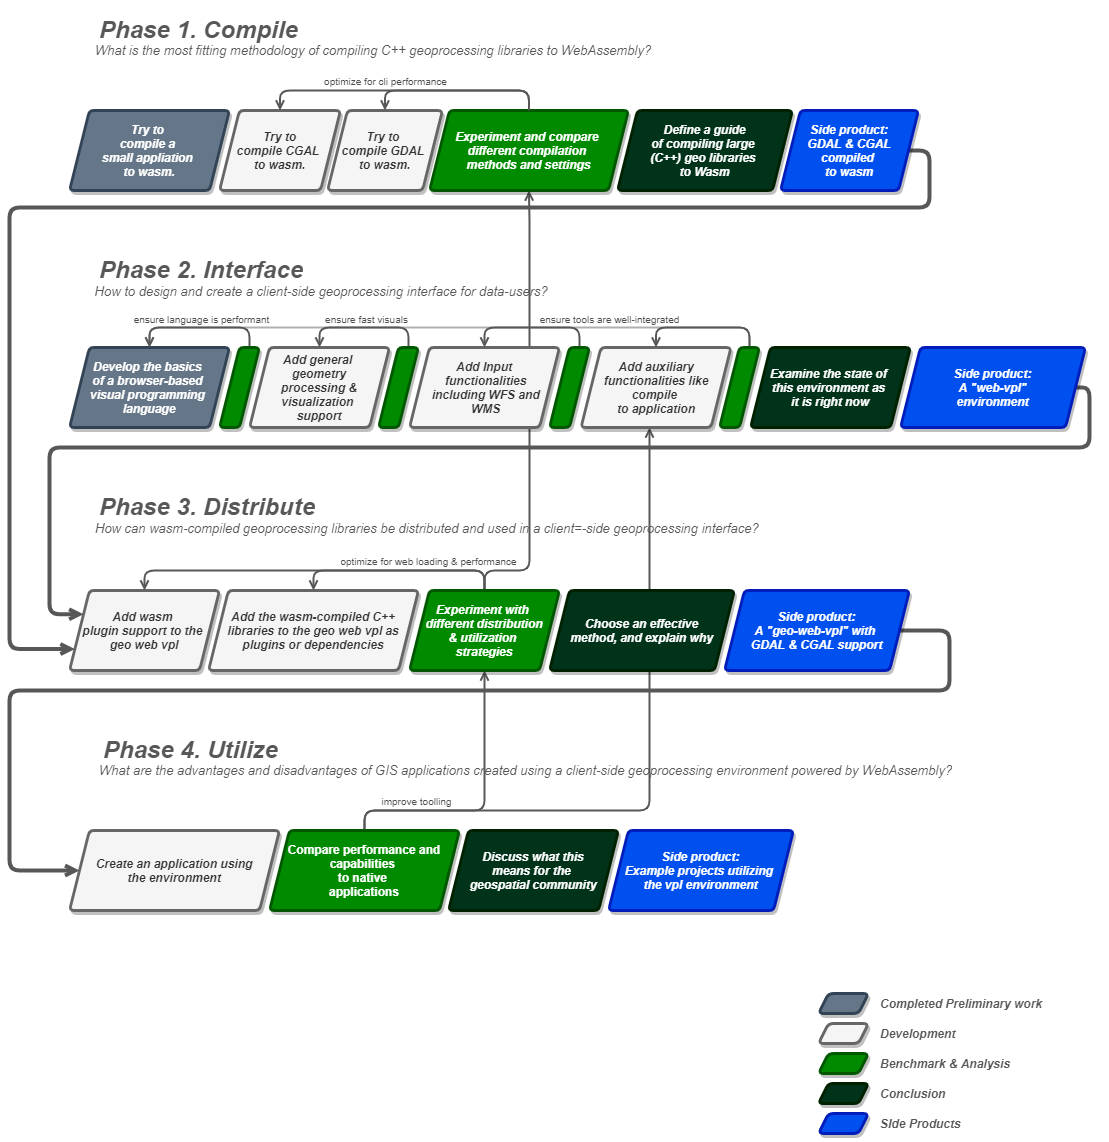
\includegraphics[width=14cm]{method.png}
    \caption{Methodology schema}
    \label{fig:method}
\end{figure}


\subsection{Phase 1: Compile}

The first phase will be about the procedure to successfully compile CGAL and GDAL to WebAssembly.

This will require research into the technicalities of the compilation target, as well as the compilation tool Emscripten (SOURCE).

The first phase will contrive of a number of steps:

- 1.1. Compile a small geoprocessing C++ script to wasm.
- 1.2  Compile CGAL \& GDAL to wasm.
- 1.3  Comparison and discussion of multiple wasm compilation methods and considerations for large libraries.


(mention preliminary work with hugo, and the knowledge gained by using WebAssembly)


\subsection{Phase 2: Develop}

% The second phase is the development of the aforementioned web-based geoprocessing tools. 

% The current plan is to shape this like a visual programming language. 

The second phase is characterized by the creation of a client-side geoprocessing environment. While all phases will entail some level of software development, this is the phase where an entire application will have to be created.

Just like the entire project, the development trajectory during phase 2 will be done incrementally, ensuring results can be produced and shown during all steps of the development. 

Creating a client-side geoprocessing application comes with many design considerations. 



Phase 2. Develop. ** a browser-based visual programming language (web-vpl), which can visualize geometry, and contains basic GIS functionalities.  


To provide an environment meant for client-side geoprocessing using WebAssembly,



A thick-client web application will be created, and this will serve as platform for testing the aforementioned ‘wagl‘’s. The tool and can be additionally used for acquiring, visualizing, and saving geodata.

At the end of this step, This environment will be usable 

basic mathematical and geometry procedures. 

and will not contain any geodata processing capabilities, nor WebAssembly. 





(mention preliminary work)

- 2D Canvas API / SVG 

- DAG : Directed Acyclic Graph

- Granular classes



\subsection{Phase 3: Synthesize}

Phase 3. Synthesize. **Combine** wasm to the environment to use the wasm-compiled CGAL and GDAL libraries.

in terms of distributing, loading, and using 
What is the optimal way of distributing, loading, and using?

hypothesis: splitting large C++ libraries up in smaller, maybe even "per function" compilation targets. 
Utilize WebAssemblies ability to accept dependencies.
Need to research more into Emscripten's capabilities.

\subsection{Phase 4: Benchmark}

The fourth phase will be a benchmarking phase. This is one of the later phases, to make use of the fact that an entire geoprocessing environment will have been created at this stage,which can then be used as a benchmarking test suite. 

The most important benchmarks that will have to be made is the comparison of the CGAL \& GDAL libraries natively versus fully integrated in the environment. Additionally, many "in-between" version are possible, which might pose valuable insight. In total, per method or functionality, five different states are of interest to this study:

\begin{itemize}
    \item Compiled and run as native binary (g++),
    \item Compiled to asm.js, run natively (node.js),
    \item Compiled to asm.js, run in a browser.
    \item Compiled to wasm, run natively (WASI),
    \item Compiled to wasm, run in a browser,
\end{itemize}



\subsection{Phase 5: Utilize}

Finally, When the VPL contains all tools necessary to be used to properly process geodata, a final assessment can be made by actually using the environment to create applications.
I hypothesize that applications equipped with client-side geoprocessing open up a whole range of new possibilities for both academic \& commercial benefits. 
I intent to discuss these aspects of the study during this phase. 



% Three different applications will be created using regular means (jupyter notebook, python, % panda's, etc)
% and these same applications will be created using the prototype web-VPL. 
% These two methods will then be compared on usability aspects and performance.   

% ## 5.3 Case Study

% > ### *Demo Application: On Demand Triangulator + Isocurves* 
% > 
% > ### Input: 
% > - Point Cloud
% > 
% > ### Output
% > - Line Curves / .png render of line curves
% > 
% > ### Steps: 
% > - Load ahn3 point-cloud (WFS Input Widget | WFS Preview Widget)
% > - Visualize point cloud on top of base map of the netherlands (WMS Input Widget | WMS > Preview Widget)
% > - Only select terrain points (list filter Operation)
% > - Construct a 2d polygon by clicking points on a map (Polygon Input Widget)
% > - Select Area of interest using a 2d polygon (Boundary Include Operation)
% > - Triangulate point cloud with a certain resolution (Triangulate Operation)
% > - Intersect the mesh surface with a series of planes (Isocurves from Mesh Operation)
% > - Preview data (MultiLine Preview Widget)
% > - Export data (MultiLine export Widget)